\documentclass{article}
\usepackage{amsmath}
\usepackage{amssymb}
\usepackage{graphicx}
\usepackage{hyperref}
\usepackage{enumitem}
\usepackage{times}
\usepackage{breqn}
\usepackage{float}
\usepackage{fancyhdr,graphicx,amsmath,amssymb}
\usepackage[ruled,vlined]{algorithm2e}
\include{pythonlisting}

\title{Algorithms Homework 8}
\author{Koi Stephanos}
\date{November 2019}

\begin{document}

\maketitle

\begin{enumerate}
\item
    Type 1 and Type 3

\item
    The main difference between LL and LR parsing is that LL parsers begin at a start symbol and work their way up to the target string we are attempting to parse while expanding non-terminals, whereas LR parsers do the opposite, and begin with our target string and try to work down or backwards until we arrive at the starting symbol, reducing non-terminals. Both construct a parsing tree, but LL pre-traverses while LR post-traverses. All this means that LL parsers work on grammars that are context-free, and LR parsers work on grammars that require context.
    
    An example of each would be a type of compiler then, but given their differences, LL works best with natural languages which are by default context-free, and LR works best with programmatic languages which are almost entirely context dependent.
    
\item
    A FSM or finite state machine is a set of states and transitions that model a particular logical flow. Here, each state our machine can be in is represented by a node, and you can only move from one state to another by a transition. A Turing machine is essentially the same, except it has a tape memory on which each transition is recorded. This means that while a finite state machine can only be in n states, where n represents the number of nodes, a Turing machine could potentially have infinite states, because you have a history of where you have been. For example, if we have a FSM and Turing machine with the same nodes and transitions, and we are at the same state in both, then all we know about the FSM is the possible state we just came from because of the linked transitions, but on the Turning machine, we have an exact history of every visited state and can glean far more about the actual operations that are occurring and can identify errors like a closed loop in our logic.

\item
    If the graph is a direct acyclic graph, that means that it can be topologically sorted. This is done be ordering the the nodes such that for every edge \(uv\) node \(u\) occurs before node \(v\) in the sorting. This sorting essentially gives us the flow through the path, as the nodes at the end are endpoints and the nodes at the beginning are our starting points. That means if something sorts correctly, there must be a flow through the network. If there were a cycle, there is no way to sort the nodes such that \(u\) always preceded \(v\). For it to be a Hamiltonian path, however, we can not visit a node more than one time, which means that each node must flow to the next. We can test this by looking at the adjacency of the nodes in our sorted list. If we can sort the nodes by edges and each pair in that sorted list is adjacent to each other, the graph can be said to have a Hamiltonian path. Here is an example of the algorithm that performs this calculation in polynomial time:
    
    \hspace*{.5em}\begin{minipage}{.99\linewidth}
        \begin{algorithm}[H]
            \SetAlgoLined
            \KwIn{nodes, edges}
            \KwResult{Returns true or false depending on whether a Hamiltonian cycle was discovered}
            \BlankLine
            sortedNodes = new Arr[nodes.length]\;
            startPoints = new Arr[nodes.length]\;
            \BlankLine
             \For{each node \(m\) in nodes}{
                    \If{\(m\) has no incoming edges}{
                        insert \(m\) into startPoints
                    }
                }
            \While{startPoints.length \(>\) 0}{
                move node \(n\) from startPoints to sortedNodes
                
                \For{each node \(m\) with an edge \(e\) from \(n\) to \(m\)}{
                    remove \(e\) from edges
                    
                    \If{\(m\) has no other incoming edges}{
                        insert \(m\) into startPoints
                    }
                }
            }
            \If{edges.length \(>\) 0}{
               return false     //We must have a cycle, so return false
            }
            \For{each pair of nodes \(n,m\)}{
                    \If{\(n\) is not adjacent to \(m\)}{
                        return false
                    }
            }
            return true
        \end{algorithm}
    \end{minipage}
\pagebreak
\item
    You can conclude that a problem is \(\epsilon P\) if it can be reduced to a different problem that is \(\epsilon P\). In the case of 2-CNF-SAT, this can be achieved by creating a graph out of the digital circuits, because we know that the graph SAT problem is NP-c.
    
    In order to satisfy a 2-CNF-SAT set up, you must not have any two chips that take \(x\) and \(~x\) as input, because if you did, there would be no way to exit the system with a 1. This can be represented as a graph by making each gate a node with two edges, each edge being an input. This mirrors the unsatisfiablity of the graph problem, because if we have to conflicting inputs to our gate, we will have a loop in our graph, where essentially we flip back and forth between 1,0 or satisfied and unsatisfied continuously. In this way we have shown that the 2-CNF-SAT problem is solvable if you can solve the SAT Graph problem, because that graph could be used to resolve the chip problem, so we can conclude that the 2-CNF-SAT problem is NP-c.

\item 
    \begin{enumerate}[label=(\alph*)]
        \item
            \(b^*(ab^+|aab^+)^*(a|aa|)\)
            
            \begin{figure}[H]
            \centerline{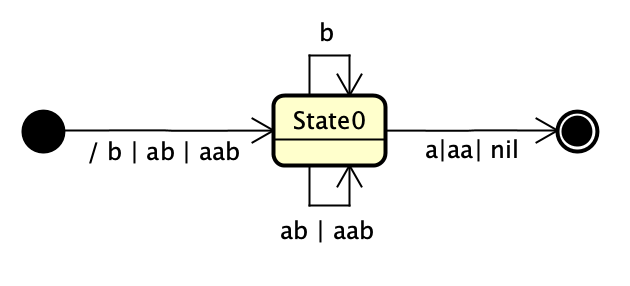
\includegraphics[width=12cm]{stateMachine.png}}
            \end{figure}

        \item
            \(0^*1?00^+\)
            
        \item
            \((10|0)^+0\)
        
        \item
            \(0^*(10^*10^*)^*\)
    \end{enumerate}
\end{enumerate}
\end{document}